% Generated by pysimcount.figleader -- do not edit; regenerate instead.
% figure: bound-min-cnot-all-formulas -- bound curves (no error bars) with n = 180..525 enlarged
% seeds [1, 2, 3, 4, 5, 6, 7, 8, 9, 10]; metric=cnot kind=xyz merged (Clifford+Rz (cz), simcount template)
% shown: suzuki2, suzuki4, mo-q6, mo-q14, bm-q10, mo-o8-q21, morales-y8m10, morales-m8
% removed (see bound-min-cnot-all-formulas-ranking.md): lie-trotter, suzuki6, suzuki8
% r from minimised norm bound (Childs et al. 2018, Def. 2; extended to every formula)
% left axis: coordinates copied unchanged from the source .tex
% right axis: the same coordinates and error bars, clipped to the window
% derived: bound-min-cnot-all-formulas.tex by pysimcount.figleader; source_sha256=3e582f6dcf655fecf58c53f4a15968836fb599e9feb244a658eb1206fc0bd2d6
% figure made at git_commit=eed0c490bd2a7ed3c821acf76ae930c79d2195f6 git_dirty=True
% WARNING: made from uncommitted code; the commit above does not reproduce it.
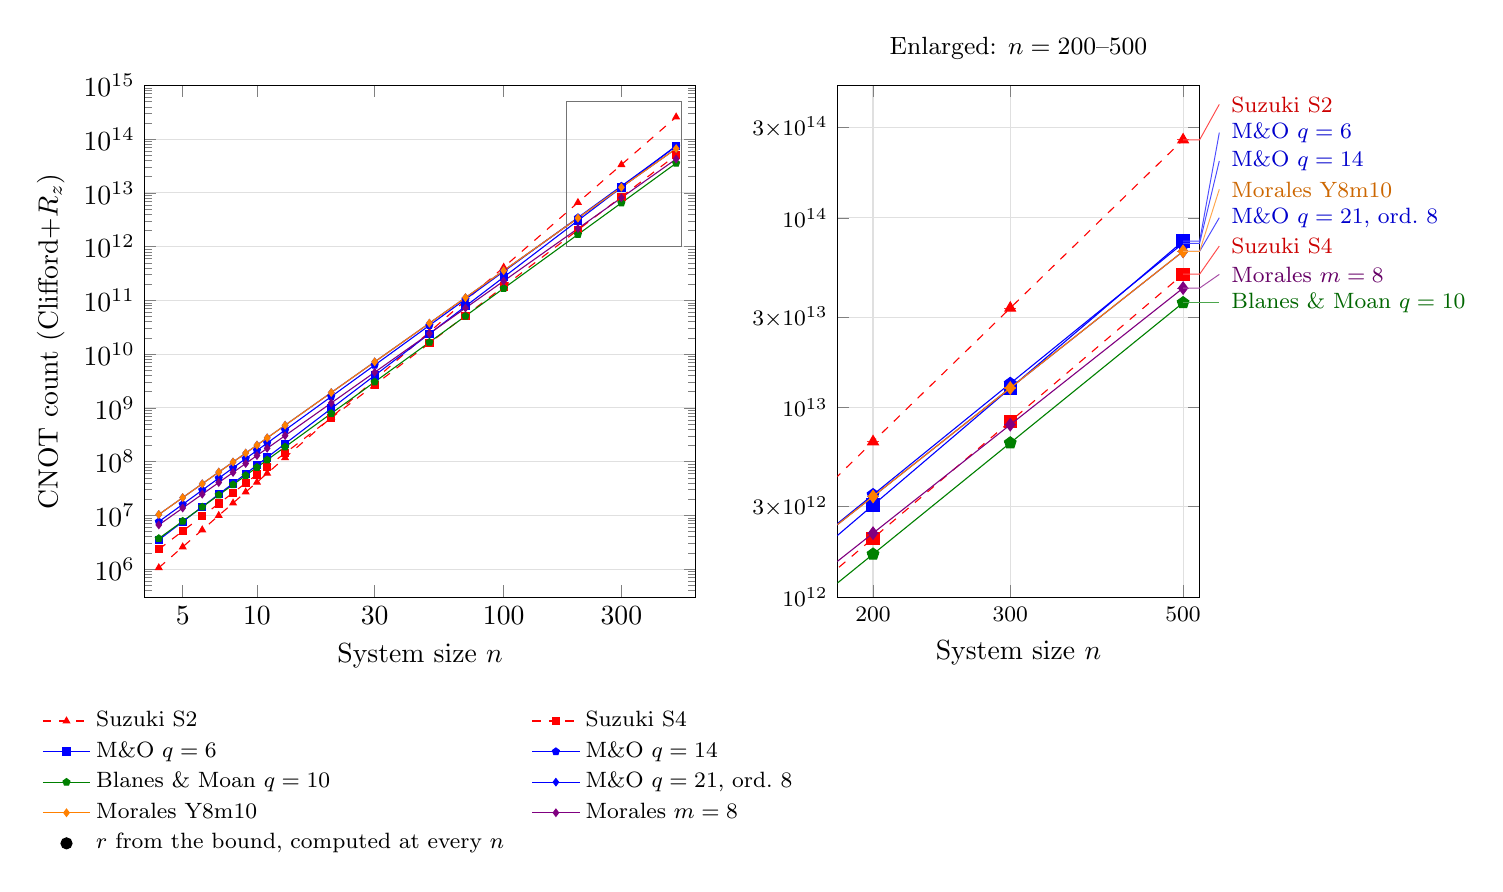
\begin{tikzpicture}
  \begin{loglogaxis}[
    name=main, scale only axis,
    width=7.0cm, height=6.5cm,
    xlabel={System size $n$},
    ylabel={CNOT count (Clifford+$R_z$)},
    xtick={5,10,30,100,300}, xticklabels={5,10,30,100,300},
    xmin=3.5, xmax=600, ymin=300000, ymax=1e+15,
    ymajorgrids=true, grid style={black!12},
    legend style={at={(0.5,-0.2)}, anchor=north, draw=none, font=\footnotesize,
      legend columns=2, /tikz/every even column/.append style={column sep=8pt}},
    legend cell align=left,
  ]
    \draw[black!55, line width=0.5pt] (axis cs:180,1e+12) rectangle (axis cs:525,5e+14);
    % suzuki2: r from the bound at every n; point = mean over seeds, bars min..max over seeds
    \addplot[red, dashed, mark=triangle*, mark size=1.3pt, mark options={solid, fill=red}] coordinates {
      (4,1.06016e+06)
      (5,2.587e+06)
      (6,5.36268e+06)
      (7,9.93272e+06)
      (8,1.69418e+07)
      (9,2.71339e+07)
      (10,4.13519e+07)
      (11,6.0538e+07)
      (13,1.18079e+08)
      (20,6.61309e+08)
      (30,3.34734e+09)
      (50,2.58249e+10)
      (70,9.92034e+10)
      (100,4.13158e+11)
      (200,6.61021e+12)
      (300,3.34637e+13)
      (500,2.58204e+14)
    };
    \addlegendentry{Suzuki S2}
    % suzuki4: r from the bound at every n; point = mean over seeds, bars min..max over seeds
    \addplot[red, dashed, mark=square*, mark size=1.3pt, mark options={solid, fill=red}] coordinates {
      (4,2.33755e+06)
      (5,5.09817e+06)
      (6,9.64202e+06)
      (7,1.65263e+07)
      (8,2.63575e+07)
      (9,3.97868e+07)
      (10,5.75064e+07)
      (11,8.02499e+07)
      (13,1.43923e+08)
      (20,6.49228e+08)
      (30,2.68105e+09)
      (50,1.6009e+10)
      (70,5.19507e+10)
      (100,1.80947e+11)
      (200,2.0458e+12)
      (300,8.45378e+12)
      (500,5.05115e+13)
    };
    \addlegendentry{Suzuki S4}
    % mo-q6: r from the bound at every n; point = mean over seeds, bars min..max over seeds
    \addplot[blue, solid, mark=square*, mark size=1.3pt, mark options={solid, fill=blue}] coordinates {
      (4,3.4934e+06)
      (5,7.61925e+06)
      (6,1.44105e+07)
      (7,2.47006e+07)
      (8,3.93952e+07)
      (9,5.94684e+07)
      (10,8.59555e+07)
      (11,1.19952e+08)
      (13,2.15132e+08)
      (20,9.70498e+08)
      (30,4.00794e+09)
      (50,2.3933e+10)
      (70,7.76668e+10)
      (100,2.70523e+11)
      (200,3.05864e+12)
      (300,1.26393e+13)
      (500,7.5521e+13)
    };
    \addlegendentry{M\&O $q=6$}
    % mo-q14: r from the bound at every n; point = mean over seeds, bars min..max over seeds
    \addplot[blue, solid, mark=pentagon*, mark size=1.3pt, mark options={solid, fill=blue}] coordinates {
      (4,7.63435e+06)
      (5,1.60415e+07)
      (6,2.94284e+07)
      (7,4.91568e+07)
      (8,7.66682e+07)
      (9,1.13471e+08)
      (10,1.61142e+08)
      (11,2.21313e+08)
      (13,3.85962e+08)
      (20,1.61983e+09)
      (30,6.24984e+09)
      (50,3.42566e+10)
      (70,1.05071e+11)
      (100,3.44736e+11)
      (200,3.47032e+12)
      (300,1.3399e+13)
      (500,7.34983e+13)
    };
    \addlegendentry{M\&O $q=14$}
    % bm-q10: r from the bound at every n; point = mean over seeds, bars min..max over seeds
    \addplot[green!50!black, solid, mark=pentagon*, mark size=1.3pt, mark options={solid, fill=green!50!black}] coordinates {
      (4,3.7123e+06)
      (5,7.79984e+06)
      (6,1.43079e+07)
      (7,2.38991e+07)
      (8,3.72726e+07)
      (9,5.51633e+07)
      (10,7.83362e+07)
      (11,1.07585e+08)
      (13,1.87617e+08)
      (20,7.87331e+08)
      (30,3.03755e+09)
      (50,1.66481e+10)
      (70,5.10601e+10)
      (100,1.6752e+11)
      (200,1.68623e+12)
      (300,6.51037e+12)
      (500,3.57103e+13)
    };
    \addlegendentry{Blanes \& Moan $q=10$}
    % mo-o8-q21: r from the bound at every n; point = mean over seeds, bars min..max over seeds
    \addplot[blue, solid, mark=diamond*, mark size=1.3pt, mark options={solid, fill=blue}] coordinates {
      (4,1.03646e+07)
      (5,2.138e+07)
      (6,3.86325e+07)
      (7,6.3709e+07)
      (8,9.82668e+07)
      (9,1.44019e+08)
      (10,2.02737e+08)
      (11,2.76236e+08)
      (13,4.75081e+08)
      (20,1.92344e+09)
      (30,7.174e+09)
      (50,3.76772e+10)
      (70,1.12353e+11)
      (100,3.57779e+11)
      (200,3.39843e+12)
      (300,1.26831e+13)
      (500,6.66564e+13)
    };
    \addlegendentry{M\&O $q=21$, ord.~8}
    % morales-y8m10: r from the bound at every n; point = mean over seeds, bars min..max over seeds
    \addplot[orange, solid, mark=diamond*, mark size=1.3pt, mark options={solid, fill=orange}] coordinates {
      (4,1.03646e+07)
      (5,2.138e+07)
      (6,3.86325e+07)
      (7,6.3709e+07)
      (8,9.82668e+07)
      (9,1.44019e+08)
      (10,2.02737e+08)
      (11,2.76236e+08)
      (13,4.75081e+08)
      (20,1.92344e+09)
      (30,7.174e+09)
      (50,3.76772e+10)
      (70,1.12353e+11)
      (100,3.57779e+11)
      (200,3.39843e+12)
      (300,1.26831e+13)
      (500,6.66564e+13)
    };
    \addlegendentry{Morales Y8m10}
    % morales-m8: r from the bound at every n; point = mean over seeds, bars min..max over seeds
    \addplot[violet, solid, mark=diamond*, mark size=1.3pt, mark options={solid, fill=violet}] coordinates {
      (4,6.6378e+06)
      (5,1.3691e+07)
      (6,2.47382e+07)
      (7,4.07951e+07)
      (8,6.29225e+07)
      (9,9.22185e+07)
      (10,1.29814e+08)
      (11,1.76874e+08)
      (13,3.04191e+08)
      (20,1.23151e+09)
      (30,4.59308e+09)
      (50,2.41214e+10)
      (70,7.19279e+10)
      (100,2.29044e+11)
      (200,2.17553e+12)
      (300,8.119e+12)
      (500,4.26685e+13)
    };
    \addlegendentry{Morales $m=8$}
    \addlegendimage{only marks, black, mark=*, mark options={solid, fill=black}}
    \addlegendentry{$r$ from the bound, computed at every $n$}
  \end{loglogaxis}
  \begin{loglogaxis}[
    scale only axis,
    at={(8.8cm,0cm)}, anchor=south west,
    width=4.6cm, height=6.5cm,
    title={Enlarged: $n = 200$--$500$}, title style={font=\small},
    xlabel={System size $n$},
    xtick={200,300,500}, xticklabels={200,300,500}, xminorticks=false,
    ytick={1e+12,3e+12,1e+13,3e+13,1e+14,3e+14}, yticklabels={{$10^{12}$},{$3{\times}10^{12}$},{$10^{13}$},{$3{\times}10^{13}$},{$10^{14}$},{$3{\times}10^{14}$}}, yminorticks=false,
    xmin=180, xmax=525, ymin=1e+12, ymax=5e+14,
    xmajorgrids=true, ymajorgrids=true, grid style={black!12}, tick label style={font=\footnotesize},
    clip mode=individual,
  ]
    % suzuki2: r from the bound at every n; point = mean over seeds, bars min..max over seeds
    \addplot[red, dashed, mark=triangle*, mark size=2.2pt, mark options={solid, fill=red}, forget plot, error bars/.cd, y dir=both, y explicit, error bar style={solid, line width=0.35pt, opacity=0.55}] coordinates {
      (4,1.06016e+06) += (0,0) -= (0,0)
      (5,2.587e+06) += (0,0) -= (0,0)
      (6,5.36268e+06) += (0,0) -= (0,0)
      (7,9.93272e+06) += (0,0) -= (0,0)
      (8,1.69418e+07) += (0,0) -= (0,0)
      (9,2.71339e+07) += (0,0) -= (0,0)
      (10,4.13519e+07) += (0,0) -= (0,0)
      (11,6.0538e+07) += (0,0) -= (0,0)
      (13,1.18079e+08) += (0,0) -= (0,0)
      (20,6.61309e+08) += (0,0) -= (0,0)
      (30,3.34734e+09) += (0,0) -= (0,0)
      (50,2.58249e+10) += (0,0) -= (0,0)
      (70,9.92034e+10) += (0,0) -= (0,0)
      (100,4.13158e+11) += (0,0) -= (0,0)
      (200,6.61021e+12) += (0,0) -= (0,0)
      (300,3.34637e+13) += (0,0) -= (0,0)
      (500,2.58204e+14) += (0,0) -= (0,0)
    };
    % suzuki4: r from the bound at every n; point = mean over seeds, bars min..max over seeds
    \addplot[red, dashed, mark=square*, mark size=2.2pt, mark options={solid, fill=red}, forget plot, error bars/.cd, y dir=both, y explicit, error bar style={solid, line width=0.35pt, opacity=0.55}] coordinates {
      (4,2.33755e+06) += (0,0) -= (0,0)
      (5,5.09817e+06) += (0,0) -= (0,0)
      (6,9.64202e+06) += (0,0) -= (0,0)
      (7,1.65263e+07) += (0,0) -= (0,0)
      (8,2.63575e+07) += (0,0) -= (0,0)
      (9,3.97868e+07) += (0,0) -= (0,0)
      (10,5.75064e+07) += (0,0) -= (0,0)
      (11,8.02499e+07) += (0,0) -= (0,0)
      (13,1.43923e+08) += (0,0) -= (0,0)
      (20,6.49228e+08) += (0,0) -= (0,0)
      (30,2.68105e+09) += (0,0) -= (0,0)
      (50,1.6009e+10) += (0,0) -= (0,0)
      (70,5.19507e+10) += (0,0) -= (0,0)
      (100,1.80947e+11) += (0,0) -= (0,0)
      (200,2.0458e+12) += (0,0) -= (0,0)
      (300,8.45378e+12) += (0,0) -= (0,0)
      (500,5.05115e+13) += (0,0) -= (0,0)
    };
    % mo-q6: r from the bound at every n; point = mean over seeds, bars min..max over seeds
    \addplot[blue, solid, mark=square*, mark size=2.2pt, mark options={solid, fill=blue}, forget plot, error bars/.cd, y dir=both, y explicit, error bar style={solid, line width=0.35pt, opacity=0.55}] coordinates {
      (4,3.4934e+06) += (0,0) -= (0,0)
      (5,7.61925e+06) += (0,0) -= (0,0)
      (6,1.44105e+07) += (0,0) -= (0,0)
      (7,2.47006e+07) += (0,0) -= (0,0)
      (8,3.93952e+07) += (0,0) -= (0,0)
      (9,5.94684e+07) += (0,0) -= (0,0)
      (10,8.59555e+07) += (0,0) -= (0,0)
      (11,1.19952e+08) += (0,0) -= (0,0)
      (13,2.15132e+08) += (0,0) -= (0,0)
      (20,9.70498e+08) += (0,0) -= (0,0)
      (30,4.00794e+09) += (0,0) -= (0,0)
      (50,2.3933e+10) += (0,0) -= (0,0)
      (70,7.76668e+10) += (0,0) -= (0,0)
      (100,2.70523e+11) += (0,0) -= (0,0)
      (200,3.05864e+12) += (0,0) -= (0,0)
      (300,1.26393e+13) += (0,0) -= (0,0)
      (500,7.5521e+13) += (0,0) -= (0,0)
    };
    % mo-q14: r from the bound at every n; point = mean over seeds, bars min..max over seeds
    \addplot[blue, solid, mark=pentagon*, mark size=2.2pt, mark options={solid, fill=blue}, forget plot, error bars/.cd, y dir=both, y explicit, error bar style={solid, line width=0.35pt, opacity=0.55}] coordinates {
      (4,7.63435e+06) += (0,0) -= (0,0)
      (5,1.60415e+07) += (0,0) -= (0,0)
      (6,2.94284e+07) += (0,0) -= (0,0)
      (7,4.91568e+07) += (0,0) -= (0,0)
      (8,7.66682e+07) += (0,0) -= (0,0)
      (9,1.13471e+08) += (0,0) -= (0,0)
      (10,1.61142e+08) += (0,0) -= (0,0)
      (11,2.21313e+08) += (0,0) -= (0,0)
      (13,3.85962e+08) += (0,0) -= (0,0)
      (20,1.61983e+09) += (0,0) -= (0,0)
      (30,6.24984e+09) += (0,0) -= (0,0)
      (50,3.42566e+10) += (0,0) -= (0,0)
      (70,1.05071e+11) += (0,0) -= (0,0)
      (100,3.44736e+11) += (0,0) -= (0,0)
      (200,3.47032e+12) += (0,0) -= (0,0)
      (300,1.3399e+13) += (0,0) -= (0,0)
      (500,7.34983e+13) += (0,0) -= (0,0)
    };
    % bm-q10: r from the bound at every n; point = mean over seeds, bars min..max over seeds
    \addplot[green!50!black, solid, mark=pentagon*, mark size=2.2pt, mark options={solid, fill=green!50!black}, forget plot, error bars/.cd, y dir=both, y explicit, error bar style={solid, line width=0.35pt, opacity=0.55}] coordinates {
      (4,3.7123e+06) += (0,0) -= (0,0)
      (5,7.79984e+06) += (0,0) -= (0,0)
      (6,1.43079e+07) += (0,0) -= (0,0)
      (7,2.38991e+07) += (0,0) -= (0,0)
      (8,3.72726e+07) += (0,0) -= (0,0)
      (9,5.51633e+07) += (0,0) -= (0,0)
      (10,7.83362e+07) += (0,0) -= (0,0)
      (11,1.07585e+08) += (0,0) -= (0,0)
      (13,1.87617e+08) += (0,0) -= (0,0)
      (20,7.87331e+08) += (0,0) -= (0,0)
      (30,3.03755e+09) += (0,0) -= (0,0)
      (50,1.66481e+10) += (0,0) -= (0,0)
      (70,5.10601e+10) += (0,0) -= (0,0)
      (100,1.6752e+11) += (0,0) -= (0,0)
      (200,1.68623e+12) += (0,0) -= (0,0)
      (300,6.51037e+12) += (0,0) -= (0,0)
      (500,3.57103e+13) += (0,0) -= (0,0)
    };
    % mo-o8-q21: r from the bound at every n; point = mean over seeds, bars min..max over seeds
    \addplot[blue, solid, mark=diamond*, mark size=2.2pt, mark options={solid, fill=blue}, forget plot, error bars/.cd, y dir=both, y explicit, error bar style={solid, line width=0.35pt, opacity=0.55}] coordinates {
      (4,1.03646e+07) += (0,0) -= (0,0)
      (5,2.138e+07) += (0,0) -= (0,0)
      (6,3.86325e+07) += (0,0) -= (0,0)
      (7,6.3709e+07) += (0,0) -= (0,0)
      (8,9.82668e+07) += (0,0) -= (0,0)
      (9,1.44019e+08) += (0,0) -= (0,0)
      (10,2.02737e+08) += (0,0) -= (0,0)
      (11,2.76236e+08) += (0,0) -= (0,0)
      (13,4.75081e+08) += (0,0) -= (0,0)
      (20,1.92344e+09) += (0,0) -= (0,0)
      (30,7.174e+09) += (0,0) -= (0,0)
      (50,3.76772e+10) += (0,0) -= (0,0)
      (70,1.12353e+11) += (0,0) -= (0,0)
      (100,3.57779e+11) += (0,0) -= (0,0)
      (200,3.39843e+12) += (0,0) -= (0,0)
      (300,1.26831e+13) += (0,0) -= (0,0)
      (500,6.66564e+13) += (0,0) -= (0,0)
    };
    % morales-y8m10: r from the bound at every n; point = mean over seeds, bars min..max over seeds
    \addplot[orange, solid, mark=diamond*, mark size=2.2pt, mark options={solid, fill=orange}, forget plot, error bars/.cd, y dir=both, y explicit, error bar style={solid, line width=0.35pt, opacity=0.55}] coordinates {
      (4,1.03646e+07) += (0,0) -= (0,0)
      (5,2.138e+07) += (0,0) -= (0,0)
      (6,3.86325e+07) += (0,0) -= (0,0)
      (7,6.3709e+07) += (0,0) -= (0,0)
      (8,9.82668e+07) += (0,0) -= (0,0)
      (9,1.44019e+08) += (0,0) -= (0,0)
      (10,2.02737e+08) += (0,0) -= (0,0)
      (11,2.76236e+08) += (0,0) -= (0,0)
      (13,4.75081e+08) += (0,0) -= (0,0)
      (20,1.92344e+09) += (0,0) -= (0,0)
      (30,7.174e+09) += (0,0) -= (0,0)
      (50,3.76772e+10) += (0,0) -= (0,0)
      (70,1.12353e+11) += (0,0) -= (0,0)
      (100,3.57779e+11) += (0,0) -= (0,0)
      (200,3.39843e+12) += (0,0) -= (0,0)
      (300,1.26831e+13) += (0,0) -= (0,0)
      (500,6.66564e+13) += (0,0) -= (0,0)
    };
    % morales-m8: r from the bound at every n; point = mean over seeds, bars min..max over seeds
    \addplot[violet, solid, mark=diamond*, mark size=2.2pt, mark options={solid, fill=violet}, forget plot, error bars/.cd, y dir=both, y explicit, error bar style={solid, line width=0.35pt, opacity=0.55}] coordinates {
      (4,6.6378e+06) += (0,0) -= (0,0)
      (5,1.3691e+07) += (0,0) -= (0,0)
      (6,2.47382e+07) += (0,0) -= (0,0)
      (7,4.07951e+07) += (0,0) -= (0,0)
      (8,6.29225e+07) += (0,0) -= (0,0)
      (9,9.22185e+07) += (0,0) -= (0,0)
      (10,1.29814e+08) += (0,0) -= (0,0)
      (11,1.76874e+08) += (0,0) -= (0,0)
      (13,3.04191e+08) += (0,0) -= (0,0)
      (20,1.23151e+09) += (0,0) -= (0,0)
      (30,4.59308e+09) += (0,0) -= (0,0)
      (50,2.41214e+10) += (0,0) -= (0,0)
      (70,7.19279e+10) += (0,0) -= (0,0)
      (100,2.29044e+11) += (0,0) -= (0,0)
      (200,2.17553e+12) += (0,0) -= (0,0)
      (300,8.119e+12) += (0,0) -= (0,0)
      (500,4.26685e+13) += (0,0) -= (0,0)
    };
    \draw[red!70, line width=0.35pt] (axis cs:500,2.58204e+14) -- (axis cs:525,2.58204e+14) -- ([xshift=0.25cm]axis cs:525,3.97341e+14);
    \node[anchor=west, font=\footnotesize, text=red!80!black] at ([xshift=0.28cm]axis cs:525,3.97341e+14) {Suzuki S2};
    \draw[red!70, line width=0.35pt] (axis cs:500,5.05115e+13) -- (axis cs:525,5.05115e+13) -- ([xshift=0.25cm]axis cs:525,7.10815e+13);
    \node[anchor=west, font=\footnotesize, text=red!80!black] at ([xshift=0.28cm]axis cs:525,7.10815e+13) {Suzuki S4};
    \draw[blue!70, line width=0.35pt] (axis cs:500,7.5521e+13) -- (axis cs:525,7.5521e+13) -- ([xshift=0.25cm]axis cs:525,2.81632e+14);
    \node[anchor=west, font=\footnotesize, text=blue!80!black] at ([xshift=0.28cm]axis cs:525,2.81632e+14) {M\&O $q=6$};
    \draw[blue!70, line width=0.35pt] (axis cs:500,7.34983e+13) -- (axis cs:525,7.34983e+13) -- ([xshift=0.25cm]axis cs:525,1.99618e+14);
    \node[anchor=west, font=\footnotesize, text=blue!80!black] at ([xshift=0.28cm]axis cs:525,1.99618e+14) {M\&O $q=14$};
    \draw[green!50!black!70, line width=0.35pt] (axis cs:500,3.57103e+13) -- (axis cs:525,3.57103e+13) -- ([xshift=0.25cm]axis cs:525,3.57103e+13);
    \node[anchor=west, font=\footnotesize, text=green!50!black!80!black] at ([xshift=0.28cm]axis cs:525,3.57103e+13) {Blanes \& Moan $q=10$};
    \draw[blue!70, line width=0.35pt] (axis cs:500,6.66564e+13) -- (axis cs:525,6.66564e+13) -- ([xshift=0.25cm]axis cs:525,1.00285e+14);
    \node[anchor=west, font=\footnotesize, text=blue!80!black] at ([xshift=0.28cm]axis cs:525,1.00285e+14) {M\&O $q=21$, ord.~8};
    \draw[orange!70, line width=0.35pt] (axis cs:500,6.66564e+13) -- (axis cs:525,6.66564e+13) -- ([xshift=0.25cm]axis cs:525,1.41488e+14);
    \node[anchor=west, font=\footnotesize, text=orange!80!black] at ([xshift=0.28cm]axis cs:525,1.41488e+14) {Morales Y8m10};
    \draw[violet!70, line width=0.35pt] (axis cs:500,4.26685e+13) -- (axis cs:525,4.26685e+13) -- ([xshift=0.25cm]axis cs:525,5.03819e+13);
    \node[anchor=west, font=\footnotesize, text=violet!80!black] at ([xshift=0.28cm]axis cs:525,5.03819e+13) {Morales $m=8$};
  \end{loglogaxis}
\end{tikzpicture}
